\documentclass[jou,apacite, 10px]{apa6}
\usepackage{listings}
\usepackage{courier}
\lstset{basicstyle=\small\ttfamily,breaklines=true}
\lstset{frame=single}
\makeatletter
\newcommand*{\rom}[1]{\expandafter\@slowromancap\romannumeral #1@}
\makeatother
\title{Classify a book's category based on its title}
\shorttitle{Book classification using book titles}

\twoauthors{Yunkai Wang}{Jules Kuehn}
\twoaffiliations{Carleton University, School of Computer Science}{Carleton University, School of Computer Science}

\abstract{Recently Convolutional neural networks(CNN) have been well-studied and be shown that they can archive incredible results on tasks like sentence classification (Kim, 2014). Another interesting topic that has been studied is if we can categorize a book based on its cover picture (Iwana et al.). However, as shown in the paper, they showed that they were able to draw a relationship between a book cover image, and its category, but the accuracy was less than $50\%$. Thus, we conduct this experiment to see if we can use CNN to learn the potential relationship between a book's title and its categories. For this project, we experiment the task with different model setups and layers using word embedding, and compare their accuracies.}

\leftheader{Jules, Yunkai}

\begin{document}
\maketitle    
                        
\section{\rom{1}. Introduction}
Book titles will given the reader a first impression of what the book may be about, and most of the time, a good book title will attract more readers from buying and reading the book. But what does the book title really tells you? What can you tell by simply looking at the book title? If a title contains the word 'calendar', then most likely people will all agree that it's a calendar, but what if the book title doesn't contain a specific word that reveals its category, like if you are given the book title 'The Three-Body Problem' with knowing this book before, how will you categorize the book? Will the book title be sufficient for a CNN that has been pre-trained with titles and categories be able to detect that as a science friction? This is a very interesting question to ask, and that's why we conduct this experiment, to see if the computers are able to learn the potential relationship between a book's title and its category using CNN.\\

\section{\rom{2}. Background/Related work}

\subsection{Dateset}
The \textit{Data Mining} is a dataset which can be found on \textit{Github.com}. The set consists of detailed information of $207572$  books from $32$ categories, to help determining the potential relationship between different information related to a book, like the relationship between a book's cover image and its category (Iwana et al.). Most of the categories are not similar to other categories, like 'calendar' and 'law', but some of the categories are pairwise similar, like 'Christian Books and Bibles' and 'Religion and Spirituality'. All books in the dataset have informations like the image url of the cover image of the book, the book's author, and the book's category. The dataset doesn't have the training dataset and testing set splitted by default, so we just use make a use of the \textit{sklearn} library, which provides a nice \textit{train\_test\_split} function to create the training set and test set.

\subsection{Loading and transforming the data}
Here are the list of things we did to load the dataset:

\rule{0pt}{4ex}  1. First we load all the original data line by line, and for each line, we extract the book title and its category, as those are the only things that we are feeding to our neural network.

\rule{0pt}{4ex}  2. It's obvious that titles all have different lengths, and the maximum title length is $96$. However, as Figure $1$ shows, most of titles have length less than $26$, only several titles have length $>26$. Therefore, we choose the maximum length to be $26$ instead of $96$. We used \textit{pad\_sequence} function from keras library to accomplish the task, which simply appends $0$ to the end of the titles that are shorter than the given length, and cut-off those long titles after $26$ words.

\rule{0pt}{4ex}  3. With the help of \textit{train\_test\_split} function, we split the training data and testing data by having a testing data of size $10\%$ of the original dataset.

\rule{0pt}{4ex}  4. We convert the titles into vector of integers, where each integer encodes to a word. We made use of the Keras' \textit{one\_hot} function to do the task. This vectorization process takes $\approx$ 2 hrs to run, therefore, we decide to store the vectorized data into a new .csv file, which we can use to train our data directly.\\

\section{\rom{3}. Problem Statement}

We want computers to be able to handle the categorization tasks for books based on book titles, such that in the future, the computer will be able to auto-categorize a new book given only its title. It's almost impossible to manually design a rule-based program, that will handle the categorization problem nicely and accurately. The titles and the categories don't have an obvious relationship which we can use to linearly separate the titles into categories. However, we can use CNN to learn the underlying relationship between the titles and the categories, that will achieve a high accuracy in the categorization task.\\

\section{\rom{4}. Model}
We began with 2 naive implementations, in which each "word vector" was an arbitrary unique integer. Each title is then a vector of these integers (one for each word), zero padded to the length of the longest title (96 words). This representation of the titles has little semantic value as the integers representing the words are arbitrary.\\
% Insert diagram of naive model
The first naive model was a fully connected MLP with the following configuration. Output size of each layer is indicated in parentheses.

\begin{itemize}
    \item Input (96)
    \item FC Sigmoid (625)
    \item FC Sigmoid (300)
    \item FC Softmax (32)
\end{itemize}\rule{0pt}{4ex}
The second naive model was based on a good model for the CIFAR-10 classification.

\begin{itemize}
    \item Input (96,1)
    \item Conv ReLU: 3 kernel, 1 stride (96,32)
    \item Conv ReLU: 3 kernel, 1 stride (96,32)
    \item Max pool: 2 kernel, 2 stride (48,32)
    \item Dropout: pKeep 0.8 (48,32)
    \item Conv ReLU: 3 kernel, 1 stride (48,64)
    \item Max pool: 2 kernel, 2 stride (24,64)
    \item Conv ReLU: 3 kernel, 1 stride (24,64)
    \item Max pool: 24 kernel, 24 stride (1,64)
    \item Dropout: pKeep 0.8 (1,64)
    \item Output Softmax (32)
\end{itemize}\rule{0pt}{4ex}
A better word representation is to embed each word in a n-dimensional space, where the position of each word reflects its meaning in relation to the other words. Each word is then represented by a dense vector of length n, with similar words having similar vectors. Similarity between words is inferred from context. Many pre-trained embeddings are available, trained through Word2Vec or GloVe on datasets pulled from Wikipedia, Twitter, or other sources. An embedding can also be trained from scratch, or initialized to a pre-trained dataset then trained further. We compare these three approaches.\\
The first embedding model trained the embeddings from scratch, using only the book titles from the training set. Note that we truncated the titles from a maximum of 96 words to 26 words. We chose 32 for the embedding dimension, based on the rule of the thumb that the embedding should be the fourth root of the vocabulary size. There were roughly 70,000 words in the training dataset, which suggest that the embedding dimension should be 16, but we found that 32 offered a slight improvement in practice.
\begin{itemize}
    \item Input (26, 1)
    \item Embedding (26, 32)
    \item Flatten (832)
    \item Dropout 0.5 (832)
    \item Output Softmax (32)
\end{itemize}
The second embedding model loaded 400,000 pre-trained 100-dimensional word-vectors from the GloVe.6B dataset. These word vectors were trained on Wikipedia and Gigaword, a newswire dataset. The model is identical to EmbedTrain except that the embeddings are pre-trained and fixed, with the embedding dimension increased to 100.\\
The third embedding model is identical to EmbedTrain except that the embeddings are initialized to the GloVe dataset as seen in EmbedGloveFixed. Embeddings are then retrained on the book titles.\\
For each of the three embedding models, we also tested 2 variations to compare the performance of MLP vs CNN on the title embeddings. The first variation adds a single fully connected (FC) layer:\\
\begin{itemize}
    \item Input (26, 1)
    \item Embedding (26, 32)
    \item Flatten (832)
    \item \textbf{FC ReLU (512)}
    \item Dropout 0.5 (512)
    \item Output Softmax (32)
\end{itemize}\rule{0pt}{4ex}
The second variation adds a single convolutional layer, followed by maxpool over the entire length:

\begin{itemize}
    \item Input (26, 1)
    \item Embedding (26, 32)
    \item \textbf{Conv ReLU: 3 kernel, 1 stride (24, 512)}
    \item \textbf{Max pool: 24 kernel, 24 stride (1, 512)}
    \item Flatten (512)
    \item Dropout 0.5 (512)
    \item Output Softmax (32)
\end{itemize}

\section{\rom{4}. Implementation}

The naive models were implemented using the course-provided cnn.py and mlp.py code. All other models were implemented in Keras, in which the code for the model is extremely concise:\\
\lstinputlisting{code/kerasModel.py}
As training the models is computationally intensive, we ran many of our tests on Google Colaboratory.\\

\section{\rom{5}. Experiment}
Eleven distinct models were tested. Each model was tuned in terms of hyperparameters and dropout layers through experimentation, so they each represent a fair example of the architecture.\\
All models were run for at least 25 epochs, with a learning rate of 0.001, a batch size of 128, and a embedding length of 32 (except in the case of using the 100-dimensional GloVe embeddings). Of the 207572 labelled data, we took 9/10 for training and 1/10 for validation.\\
The results of the naive model, in which no meaning is embedded in the input vector, were predictably poor. The MLP achieved only 9\% validation accuracy, while the CNN eventually reached 12\%. While these accuracies are better than chance (1/32), they are far from useful. There needs to be a meaningful representation of the input words in the input vectors, not arbitrary word indices.\\
Adding an embedding layer drastically improved the results. The best 7 models performed very similarly, all falling between 62 and 66\%.
\begin{figure}[h!]
    \centering
     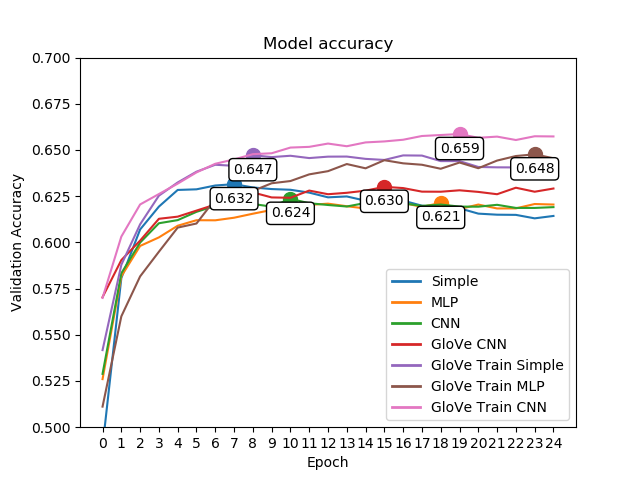
\includegraphics[width=0.5\textwidth]{images/good_models_comparison_small}
        \caption{Categorization accuracy for 7 best models}
\end{figure}


\subsection{Training embeddings from dataset}
The simple model
The MLP model
The CNN model

\subsection {Using pre-trained GloVe embeddings}
The simple model
The MLP model
The CNN model

\subsection {Re-training GloVe embeddings from dataset}
The simple model
The MLP model
The CNN model


\section{\rom{6}. Conclusion}
a
\section{References}
\noindent Convolutional Neural Networks for Sentence Classification By Yoon Kim\\
Judging a Book by its Cover By Brian et al.

\end{document}
